%\documentstyle[epsf,twocolumn]{jarticle}       %LaTeX2e仕様
%\documentclass[twocolumn]{jarticle}     %pLaTeX2e仕様(platex.exeの場合)
\documentclass[onecolumn]{ujarticle}   %pLaTeX2e仕様(uplatex.exeの場合)
%%%%%%%%%%%%%%%%%%%%%%%%%%%%%%%%%%%%%%%%%%%%%%%%%%%%%%%%%%%%%%
%%
%%  基本バージョン
%%
%%%%%%%%%%%%%%%%%%%%%%%%%%%%%%%%%%%%%%%%%%%%%%%%%%%%%%%%%%%%%%%%
\setlength{\topmargin}{-45pt}
%\setlength{\oddsidemargin}{0cm}
\setlength{\oddsidemargin}{-7.5mm}
%\setlength{\evensidemargin}{0cm}
\setlength{\textheight}{24.1cm}
%setlength{\textheight}{25cm}
\setlength{\textwidth}{17.4cm}
%\setlength{\textwidth}{172mm}
\setlength{\columnsep}{11mm}

%\kanjiskip=.07zw plus.5pt minus.5pt

% 【節が変わるごとに (1.1)(1.2) … (2.1)(2.2) と数式番号をつけるとき】
%\makeatletter
%\renewcommand{\theequation}{%
%\thesection.\arabic{equation}} %\@addtoreset{equation}{section}
%\makeatother

%\renewcommand{\arraystretch}{0.95} 行間の設定
%%%%%%%%%%%%%%%%%%%%%%%%%%%%%%%%%%%%%%%%%%%%%%%%%%%%%%%%
%\usepackage{graphicx}   %pLaTeX2e仕様(\documentstyle ->\documentclass)
\usepackage[dvipdfmx]{graphicx}
\usepackage{subcaption}
\usepackage{multirow}
\usepackage{amsmath}
\usepackage{url}
\usepackage[bb=boondox]{mathalfa}
\usepackage{listings}
\newcommand{\argmax}{\mathop{\rm arg~max}\limits}
\newcommand{\argmin}{\mathop{\rm arg~min}\limits}

\lstset{%
  language={Python},
  basicstyle={\small},%
  identifierstyle={\small},%
  commentstyle={\small\itshape},%
  keywordstyle={\small\bfseries},%
  ndkeywordstyle={\small},%
  stringstyle={\small\ttfamily},
  frame={tb},
  breaklines=true,
  columns=[l]{fullflexible},%
  numbers=left,%
  xrightmargin=0zw,%
  xleftmargin=3zw,%
  numberstyle={\scriptsize},%
  stepnumber=1,
  numbersep=1zw,%
  lineskip=-0.5ex%
}

%%%%%%%%%%%%%%%%%%%%%%%%%%%%%%%%%%%%%%%%%%%%%%%%%%%%%%%%
\begin{document}

	%bibtex用の設定
	%\bibliographystyle{ujarticle}
	\noindent

	\hspace{1em}
	2020 年 7 月 17 日
	ゼミ資料
	\hfill
	M2 寺内 光

	\vspace{2mm}

	\hrule

	\begin{center}
		{\Large \bf 進捗報告}
	\end{center}

	\hrule
	\vspace{3mm}

	% ‚ここから 文章 Start!
	\section{今週やったこと}
	\begin{itemize}{
    \item{TDGAとSGAを用いた FastAutoAugment 実験}
	}\end{itemize}
	\section{TDGAとSGAを用いた FastAutoAugment 実験}
  先週の話にあがっていた諸パラメータを以下で設定して実験を回した.
  \begin{itemize}
    \item{遺伝子表現:ビットエンコーディング}
    \item{個体数と世代数の調整:個体数16(SGAでは32),50世代}
    \item{突然変異の選択: ビット反転.突然変異率は 0.02(SGAでは0.05).ナップサックの値をそのまま使っているだけなので調整の余地あり}
    \item{初期温度の選択,温度スケジューラの導入: 初期温度 0.1,終了温度 0.02, 温度スケジューラ:指数スケジューラ}
    \item{lossの最小化かaccの最大化か: accの最大化}
    \item{最終的にどの拡張を採用するか: SGA:各探索において最良個体を保存し,あとで結合. TDGA:各探索において選択操作により何個体か選択し,あとで結合}
  \end{itemize}

  その他,適用強度については RandAugment の拡張範囲(各操作に対して上限と下限を設定し,[0, 30]でスケール)を採用した操作集合に対し,全操作の強度を統一した.また,操作集合は [
        AutoContrast,
        Equalize,
        Invert,
        Rotate,
        Posterize,
        Solarize,
        SolarizeAdd,
        Color,
        Contrast,
        Brightness,
        Sharpness,
        ShearX,
        ShearY,
        CutoutAbs,
        TranslateXabs,
        TranslateYabs
    ]
    である.各操作を 0,15,30の強度で適用した例を下に示す.ただし,AutoContrast, Equalize, Invert は強度によらない.

    \begin{figure}[h]
  		\begin{center}
  			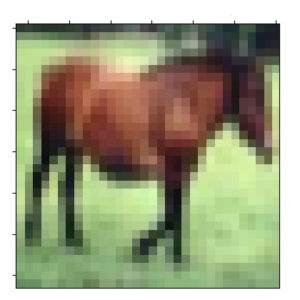
\includegraphics[width=0.3\columnwidth]{transform_test/horse.jpg}
  			\caption{元画像}
  			\label{fig:horse_original}
  		\end{center}
  	\end{figure}

    \begin{figure}[h]
      \vspace{-4mm}
      \centering
      \begin{subfigure}{0.3\columnwidth}
        \centering
        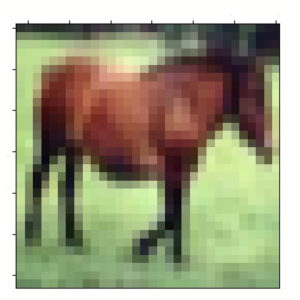
\includegraphics[width=1.0\columnwidth]{transform_test/AutoContrast_0.png}
        \caption{mag=0}
        \label{fig:AutoContrast_0}
      \end{subfigure}
      \begin{subfigure}{0.3\columnwidth}
        \centering
        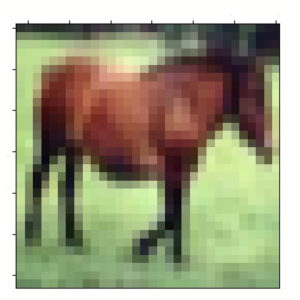
\includegraphics[width=1.0\columnwidth]{transform_test/AutoContrast_15.png}
        \caption{mag=15}
        \label{fig:AutoContrast_15}
      \end{subfigure}
      \begin{subfigure}{0.3\columnwidth}
        \centering
        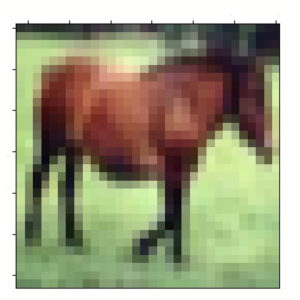
\includegraphics[width=1.0\columnwidth]{transform_test/AutoContrast_30.png}
        \caption{mag=30}
        \label{fig:AutoContrast_30}
      \end{subfigure}
      \caption{強度を変えた各操作の適用例}
      \label{fig:OperationsWithVariousMagnitude}
    \end{figure}




  \subsection{SGA}
  SGA においては交叉に1点交叉,選択にトーナメント戦略(サイズ2)を用いた.適用強度を変化させながら実験した結果,全ての探索においてどの拡張も採用しない個体が最も上位の適応度を持っていた.これに関しては元々学習している子モデルが拡張なしで学習しているためだと考えられる.
  下に探索結果の一例を示す.

  \begin{figure}[h]
		\begin{center}
			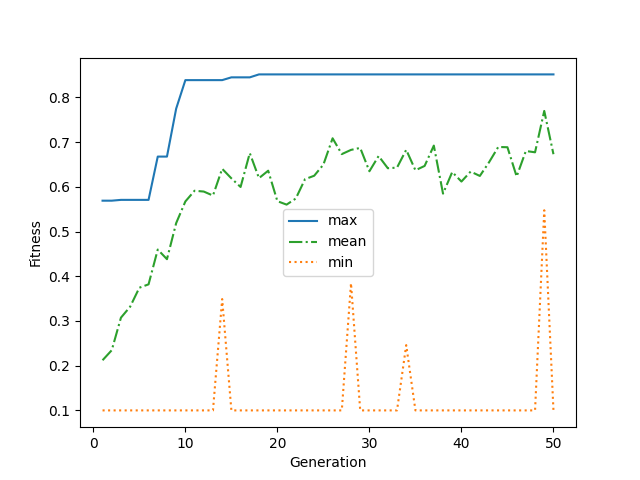
\includegraphics[width=0.7\columnwidth]{stats_SGA.png}
			\caption{SGAにおける探索の過程}
			\label{fig:SGA_stats}
		\end{center}
	\end{figure}

  \begin{figure}[h]
		\begin{center}
			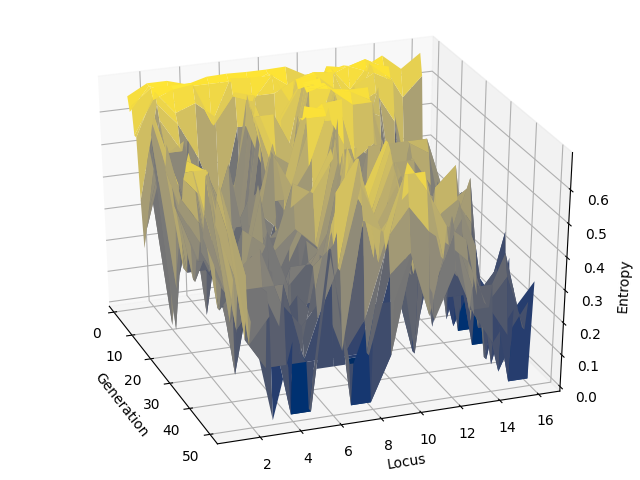
\includegraphics[width=0.7\columnwidth]{entropy_SGA.png}
			\caption{SGAにおける遺伝子座毎のエントロピー}
			\label{fig:SGA_entropy}
		\end{center}
	\end{figure}

  また,このとき Validation Accuracy は 91.240% となった.

  \subsection{TDGA}
  TDGA においては交叉に一様交叉を用いた.TDGA では多様性を維持しつつ大域解を探索することができる特徴があるので,ベイズアプローチにおいて8回探索している(子モデルの学習4回,各子モデルに対し2回のベイズ探索)ところを1回に減らして(子モデルの学習1回,子モデルに対し1回のGA探索)探索において上位8個体を採用するという方針で実験をした.ちなみにこの時点で FastAutoAugment とは何の関連性もなくなった.また,強度は 10 とし,初期温度は1(やや高い気もする),終了温度は0.02と設定した.温度スケジューラについては森先生の論文中の静的環境の対するスケジューリング関数と動的環境に対する Feedback TDGA(FTDGA) を読んだ結果,今回の問題は静的環境で指数スケジューリングを採用しているという点で現実装のままで問題なさそうだったのでひとまずこのままにしている.FTDGA の静的環境における有効性も示されてはいたが,実装コストの面で一旦保留.

  結果,この条件において FastAutoAugment と同程度の実行時間で終了した(3時間ちょっと).
  下に探索結果の一例を示す.

  \begin{figure}[h]
		\begin{center}
			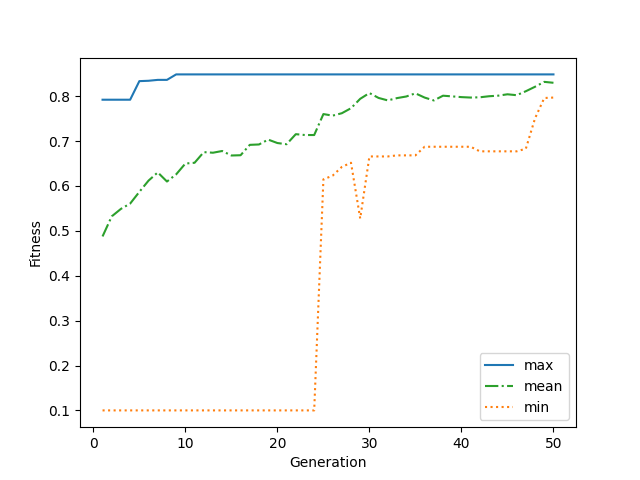
\includegraphics[width=0.7\columnwidth]{stats_TDGA.png}
			\caption{TDGAにおける探索の過程}
			\label{fig:TDGA_stats}
		\end{center}
	\end{figure}

  \begin{figure}[h]
		\begin{center}
			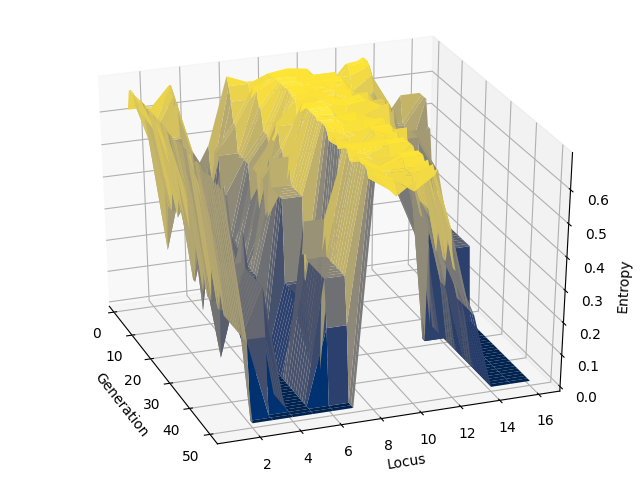
\includegraphics[width=0.7\columnwidth]{entropy_TDGA.png}
			\caption{TDGAにおける遺伝子座毎のエントロピー}
			\label{fig:TDGA_entropy}
		\end{center}
	\end{figure}

  探索が進んでいること,および温度のスケジューリングにより個体群がある遺伝子座において収束をしていることがわかる.また,このとき Validation Accuracy は 91.370% となった.また,元のレポジトリの FastAutoAugment では  91.810% の精度が出ていた.この精度がどれくらい伸びるかは適用強度,突然変異率,温度パラメータ等を変化させながら観察したい.

  また,このとき選択された操作は下のようになった.
  \lstinputlisting[caption=subpolicies\_TDGA]{subpolicies_TDGA.txt}

  拡張なしが最も高い適応度を示すのはSGAと同じだが,しっかりと多様性を維持しつつ最終的なポリシーが得られていることがわかる.しかしながら,選ばれている操作はかなり限定的であり,おおよそ元の画像に変化を加えないような操作が選ばれることがわかった.これをどう改善していくかは今後の課題になりそう.ただ,元のFastAutoAugmentではしっかり変形等の拡張が採用されていた.これはおそらくベイズ探索の強度を下げてあまりロスの下がりすぎない操作を大域的に探しているからだと考えられる.実際に探索結果の Validation Accuracy は 0.4−0.6 とそこまで良くないものが採用されていることがわかった(ただし,ベイズでやってるのはロスの最小化なので Accuracy が目的関数ではない).TDGA においても遺伝子空間の多様性に加えてこのあたりの表現空間の多様性を維持する方法を取り入れたいという感じがした.

	\section{来週のタスク}
	TDGA の適用強度と初期温度,終了温度を変化させたときの影響を観察する.

	% 参考文献リスト
	% \bibliographystyle{unsrt}
	% \bibliography{2020_07_17}
\end{document}
